\documentclass{article}

\usepackage{amsmath}
\usepackage{amsthm}
\usepackage{amssymb}

\usepackage{tikz}
\usetikzlibrary{arrows.meta, decorations.markings}

\usepackage{graphicx}

\usepackage{hyperref}
\hypersetup{
  pdftitle  = {Mathematical Accessibility Test},
  pdfauthor = {Ettore Aldrovandi},
}

\newtheorem{theorem}{Theorem}[section]
\newtheorem{definition}[theorem]{Definition}
\newtheorem{corollary}[theorem]{Corollary}

\begin{document}

\title{Mathematical Accessibility Test}
\author{Ettore Aldrovandi}
\date{\today}
\maketitle

\section{Introduction}

This document tests PDF/UA-2 accessibility tagging for mathematical content and figures.
Mathematics pervades science: the famous Euler identity $e^{i\pi} + 1 = 0$ encapsulates
the relationship between the five most important constants in mathematics.  Similarly,
the Gaussian integral
$\int_{-\infty}^{\infty} e^{-x^2}\,dx = \sqrt{\pi}$
appears throughout probability theory and physics.

The interplay between algebra and analysis has driven much of modern mathematics.
Formulae such as these encode deep structural relationships that underpin fields
ranging from quantum mechanics to probability theory. Making such content accessible
to all readers---including those relying on assistive technologies---is both a
technical challenge and an ethical imperative for mathematical publishing.

This document samples several areas of classical mathematics: elementary identities,
complex analysis via the residue theorem, and differential geometry via Stokes'
theorem. Each section pairs formal definitions and theorem statements with illustrative
computations. The final section demonstrates the inclusion of figures alongside tagged
mathematical text, exercising the full range of PDF/UA-2 accessibility features.

\section{Mathematical Formulas}

\subsection{Display Equations}

The Gaussian integral evaluates to:
\begin{equation}
  \int_{-\infty}^{\infty} e^{-x^2}\,dx = \sqrt{\pi}.
\end{equation}

The geometric series converges for $|x| < 1$:
\begin{equation}
  \sum_{k=0}^{\infty} x^k = \frac{1}{1-x}.
\end{equation}

\subsection{Aligned Equations}

The binomial identities follow from expanding $(a \pm b)^2$:
\begin{align}
  (a + b)^{2}      &= a^{2} + 2ab + b^{2},      \\
  (a - b)^{2}      &= a^{2} - 2ab + b^{2},      \\
  (a + b)(a - b)   &= a^{2} - b^{2}.
\end{align}

Identities of this kind recur throughout algebra and combinatorics, and generalise
naturally to polynomial rings and other algebraic structures. The transition from
scalar arithmetic to matrix arithmetic preserves much of this structure, though one
must take care: unlike real numbers, matrices do not in general commute under
multiplication, so the order of factors matters.

\subsection{Matrices}

A general $2 \times 2$ matrix and its determinant:
\begin{equation}
  A = \begin{pmatrix} a & b \\ c & d \end{pmatrix}, \qquad
  \det(A) = ad - bc.
\end{equation}

\section{The Residue Theorem}

Complex analysis studies functions $f\colon U \to \mathbb{C}$ that are differentiable
in the complex sense, known as \emph{holomorphic} functions. Such functions are
extraordinarily rigid: holomorphicity on an open set implies infinite differentiability
and a convergent power series representation. Isolated points where this regularity
breaks down are called \emph{singularities}, and their local behaviour is captured
precisely by the Laurent series expansion.

\begin{definition}
  Let $f$ be holomorphic on a punctured disk $0 < |z - a| < r$.  The \emph{residue}
  of $f$ at $a$ is the coefficient $a_{-1}$ in the Laurent expansion
  \begin{equation}
    f(z) = \sum_{n=-\infty}^{\infty} a_n (z - a)^n,
  \end{equation}
  equivalently,
  \begin{equation}
    \operatorname{Res}(f, a)
      = \frac{1}{2\pi i} \oint_{|z-a|=\varepsilon} f(z)\,dz.
  \end{equation}
  For a simple pole, the residue simplifies to
  \begin{equation}
    \operatorname{Res}(f, a) = \lim_{z \to a}(z - a)f(z).
  \end{equation}
\end{definition}

\begin{theorem}[Residue Theorem]
  Let $U \subset \mathbb{C}$ be open and $f$ holomorphic on $U$ except at finitely many
  isolated singularities $a_1, \ldots, a_n \in U$.  For any positively oriented simple
  closed contour $\gamma$ in $U$ avoiding all $a_k$,
  \begin{equation}
    \oint_{\gamma} f(z)\,dz
      = 2\pi i \sum_{k=1}^{n} n(\gamma, a_k)\,\operatorname{Res}(f, a_k),
  \end{equation}
  where $n(\gamma, a_k)$ denotes the winding number of $\gamma$ about $a_k$.
\end{theorem}

\subsection{Example}

Evaluate $\displaystyle I = \oint_{|z|=2} \dfrac{dz}{z^{2} - 1}$.

The integrand has simple poles at $z = \pm 1$, both enclosed by $|z| = 2$. Computing
each residue:
\begin{align}
  \operatorname{Res}\!\left(\tfrac{1}{z^{2}-1},\; 1\right)
    &= \lim_{z \to 1}  \frac{z - 1}{z^{2}-1}
     = \lim_{z \to 1}  \frac{1}{z+1}
     = \phantom{-}\frac{1}{2}, \\[4pt]
  \operatorname{Res}\!\left(\tfrac{1}{z^{2}-1},\; {-1}\right)
    &= \lim_{z \to -1} \frac{z + 1}{z^{2}-1}
     = \lim_{z \to -1} \frac{1}{z-1}
     = -\frac{1}{2}.
\end{align}
The residues sum to zero, so $I = 2\pi i \cdot 0 = 0$.

The residue theorem is one of the most powerful computational tools in complex
analysis, reducing contour integrals over closed curves to finite algebraic sums.
Its applications extend well beyond pure mathematics: it underlies partial fraction
methods in signal processing, closed-form evaluation of real improper integrals,
and aspects of the spectral theory of linear operators. The next section turns to
a related but broader integration theorem, formulated in the language of differential
forms on smooth manifolds.

\section{Stokes' Theorem}

Stokes' theorem is the central result of the calculus of differential forms,
unifying the classical theorems of Green, Gauss, and Stokes under a single statement.
Its formulation requires the language of smooth manifolds and the exterior derivative
$d$, which generalises the gradient, curl, and divergence of vector calculus to
arbitrary dimension and codimension.

\begin{theorem}[Stokes' Theorem --- General Form]
  Let $\Omega$ be a smooth oriented $k$-manifold with boundary $\partial\Omega$,
  and let $\omega$ be a smooth $(k-1)$-form on $\Omega$.  Then
  \begin{equation}
    \int_{\partial\Omega} \omega = \int_{\Omega} d\omega,
  \end{equation}
  where $d$ denotes the exterior derivative.
\end{theorem}

In classical vector calculus, taking $\Omega$ to be a surface $S \subset \mathbb{R}^{3}$
with boundary curve $\partial S$ and $\omega = \mathbf{F} \cdot d\mathbf{r}$ recovers
the familiar vector form:
\begin{equation}
  \oint_{\partial S} \mathbf{F} \cdot d\mathbf{r}
    = \iint_{S} (\nabla \times \mathbf{F}) \cdot d\mathbf{S}.
\end{equation}

\begin{corollary}[Green's Theorem]
  For a positively oriented simple closed curve $\partial D$ bounding a region
  $D \subset \mathbb{R}^{2}$ and smooth functions $P$, $Q$,
  \begin{equation}
    \oint_{\partial D} \bigl(P\,dx + Q\,dy\bigr)
      = \iint_{D} \left(\frac{\partial Q}{\partial x}
                       - \frac{\partial P}{\partial y}\right)dx\,dy.
  \end{equation}
\end{corollary}

The theorems presented in the preceding sections are best understood through geometric
intuition: closed contours winding around singularities in the complex plane, and
surfaces bounded by oriented curves in three-dimensional space. The figures below
provide visual anchors for these analytic statements, illustrating the two principal
geometric settings encountered in this document.

\section{Figures}

\subsection{Contour in the Complex Plane}

Figure~\ref{fig:contour} illustrates the setup of the Residue Theorem: a positively
oriented circular contour $\gamma$ enclosing the poles of $f(z) = 1/(z^{2}-1)$
at $z = \pm 1$.

\begin{figure}[htbp]
  \centering
  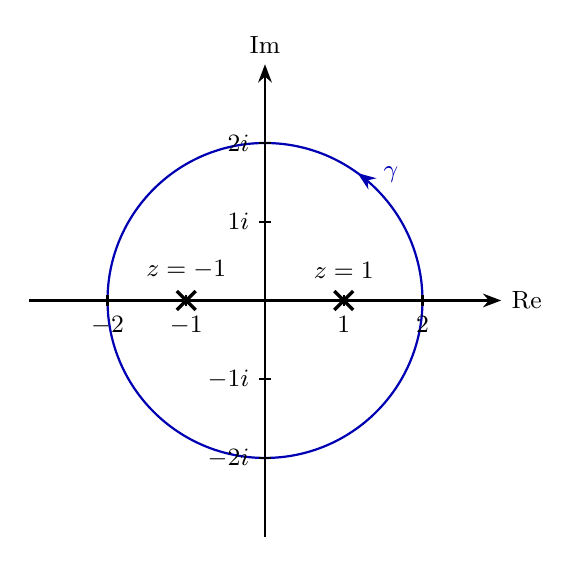
\begin{tikzpicture}[>=Stealth, thick, font=\small]
    % Axes
    \draw[->] (-3,0) -- (3,0) node[right] {$\operatorname{Re}$};
    \draw[->] (0,-3) -- (0,3) node[above] {$\operatorname{Im}$};
    % Contour (radius 2), counter-clockwise arrow at top-right
    \draw[blue!70!black, postaction={decorate,
          decoration={markings,
            mark=at position 0.15 with {\arrow{>}}}}]
      (0,0) circle (2);
    \node[blue!70!black] at (1.6,1.6) {$\gamma$};
    % Poles marked with x
    \foreach \px/\lbl in {1/{z=1}, -1/{z=-1}} {
      \draw[black, very thick]
        (\px-0.12,-0.12) -- (\px+0.12,0.12)
        (\px-0.12, 0.12) -- (\px+0.12,-0.12);
      \node[black, above] at (\px, 0.15) {$\lbl$};
    }
    % Tick marks
    \foreach \x in {-2,-1,1,2} {
      \draw (\x, 2pt) -- (\x,-2pt) node[below] {$\x$};
    }
    \foreach \y in {-2,-1,1,2} {
      \draw (2pt,\y) -- (-2pt,\y) node[left] {$\y i$};
    }
  \end{tikzpicture}
  \caption{Positively oriented contour $\gamma\colon |z|=2$ enclosing the poles
           of $1/(z^{2}-1)$ at $z = \pm 1$ (marked $\times$).}
  \label{fig:contour}
\end{figure}

\subsection{Surface with Boundary}

In the setting of Stokes' theorem, the surface $S$ may be any smooth oriented
$2$-manifold with boundary. The boundary $\partial S$ inherits an orientation from
that of $S$, conventionally determined by the right-hand rule relative to the outward
normal. The precise shape of $S$ is immaterial to the theorem---only the relationship
between $S$ and $\partial S$ governs the equality of the two integrals.

Figure~\ref{fig:stokes} depicts a surface $S$ with boundary $\partial S$,
the geometric setting of Stokes' theorem.

\begin{figure}[htbp]
  \centering
  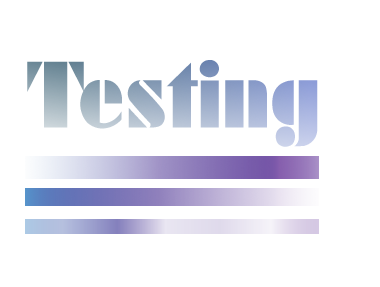
\includegraphics[width=0.5\linewidth]{alphatest}
  \caption{A surface $S$ with boundary $\partial S$ (placeholder).}
  \label{fig:stokes}
\end{figure}

\end{document}
